\documentclass{article}
\usepackage[top=2cm, bottom=2cm, left=3cm, right=3cm]{geometry}
\usepackage{amsmath}
\usepackage{physics}
\usepackage{esvect}
\usepackage{graphicx}
\usepackage{tikz}
\usepackage{siunitx}
\usepackage{tikz-3dplot}
\usepackage{subcaption}
\usepackage{siunitx}
\usepackage{booktabs}
\usepackage{array}
\usetikzlibrary{decorations.pathmorphing}
\usetikzlibrary{decorations.markings}
\usetikzlibrary{arrows}
\usetikzlibrary{arrows.meta}
\usetikzlibrary{calc}
\usetikzlibrary{patterns}
\usetikzlibrary{angles}
\usetikzlibrary{quotes}

\begin{document}

\section{Elastic Collision Derivation}
\setcounter{equation}{0}
\begin{gather}
    m_1 v_1 + m_2 v_2 = m_1 v_1' + m_2 v_2' \\
    \frac{1}{2}m_1 v_1^2 + \frac{1}{2}m_2 v_2^2 = \frac{1}{2}m_1 v_1'^2 + \frac{1}{2}m_2 v_2'^2 \\
    v_{a1} + v_{b1} = v_{a2} + v_{b2} \\
    \boxed{v_1' = \frac{(m_1 - m_2)v_1 + 2m_2 v_2}{m_1 + m_2}} \\
    \boxed{v_2' = \frac{(m_2 - m_1)v_2 + 2m_1 v_1}{m_1 + m_2}}
\end{gather}

\section{Kinematic Equations for Rigid Body Rotation}
\setcounter{equation}{0}
\begin{gather}
    \alpha = \frac{d\omega}{dt} \implies \int_{\omega_0}^\omega d\omega = \int_0^t \alpha \, dt \\
    \omega = \omega_0 + \alpha t \iff \boxed{v = v_0 + at} \\
    \frac{d\theta}{dt} = \omega_0 + \alpha t \implies \int_{\theta_0}^\theta d\theta = \int_0^t (\omega_0 + \alpha t) \, dt \\
    \theta - \theta_0 = \omega_0 t + \frac{1}{2} \alpha t^2 \iff \boxed{s = v_0 t+\frac{1}{2} at^2} \\
    \alpha = \omega \frac{d\omega}{d\theta} \implies \int_{\omega_0}^\omega \omega \, d\omega = \int_{\theta_0}^\theta \alpha \, d\theta \\
    \omega^2 - \omega_0^2 = 2 \alpha (\theta - \theta_0) \iff \boxed{v^2 - v_0^2 = 2as}
\end{gather}

\section{Particle Motion VS Rigid Body Rotation}
\begin{center}
\renewcommand{\arraystretch}{2}
\begin{tabular}{|l|l|l|l|}
\hline
\textbf{Quantity} & \textbf{Particle Motion} & \textbf{Quantity} & \textbf{Rigid Body Rotation} \\
\hline
Velocity & $\vv{v} = \dfrac{d\vv{r}}{dt}$ & Angular velocity & $\vv{\omega} = \dfrac{d\vv{\theta}}{dt}$ \\
\hline
Acceleration & $\vv{a} = \dfrac{d\vv{v}}{dt}$ & Angular acceleration & $\vv{\alpha} = \dfrac{d\vv{\omega}}{dt}$ \\
\hline
Force & $\vv{F} = m\vv{a}$ & Torque & $\vv{M} = J\vv{\alpha}$ \\
\hline
Inertia & Mass $m$ & Inertia & Moment of inertia $J = \displaystyle\int r^2 dm$ \\
\hline
Momentum & $\vv{p} = m\vv{v}$ & Angular momentum & $\vv{L} = J\vv{\omega}$ \\
\hline
Law & $\vv{F} = \dfrac{d\vv{p}}{dt}$ & Law & $\vv{M} = \dfrac{d\vv{L}}{dt}$ \\
\hline
Impulse & $\displaystyle\int \vv{F} dt = \Delta \vv{p}$ & Angular impulse & $\displaystyle\int \vv{M} dt = \Delta \vv{L}$ \\
\hline
Energy & $T = \dfrac{1}{2}mv^2$ & Rotational energy & $T = \dfrac{1}{2}J\omega^2$ \\
\hline
Work & $W = \displaystyle\int \vv{F} \cdot d\vv{r}$ & Rotational work & $W = \displaystyle\int \vv{M} \cdot d\vv{\theta}$ \\
\hline
Work-energy & $W = \dfrac{1}{2}mv_1^2 - \dfrac{1}{2}mv_2^2$ & Work-energy & $W = \dfrac{1}{2}J\omega_1^2 - \dfrac{1}{2}J\omega_2^2$ \\
\hline
\end{tabular}
\end{center}

\newpage

\section{Problem}
Find the moment of inertia for the following physical models using the advanced mathematical definition of moment of inertia:
\begin{enumerate}
    \item Thin rod of length $l$, rotation axis through center perpendicular to rod.
    \item Cylinder of radius $R$, rotation axis along geometric axis.
    \item Thin ring of radius $R$, rotation axis along geometric axis.
    \item Sphere of radius $R$, rotation axis along any diameter.
    \item Cylindrical shell with outer radius $R_2$, inner radius $R_1$, rotation axis along geometric axis.
    \item Thin rod of length $l$, rotation axis through one end perpendicular to rod.
\end{enumerate}
\section*{Solution}
\setcounter{equation}{0}
\begin{enumerate}
    \item Thin rod (center axis):
    \begin{gather}
        J = \int_{-l/2}^{l/2} r^2 \lambda \, dr = \lambda \left[ \frac{r^3}{3} \right]_{-l/2}^{l/2} = \frac{\lambda l^3}{12} = \boxed{\frac{m l^2}{12}}
    \end{gather}
    \begin{tikzpicture}
        \draw[thick] (0,0) -- (4,0);
        \draw[thick, dashed] (-2,0) -- (0,0);
        \draw[->] (2,1) -- (2,2) node[above] {$\vv{P}$};
        \draw[dashed] (2,0) -- (2,1);
        \draw[<->] (0,-0.5) -- (4,-0.5) node[midway,below] {$l$};
        \draw[fill] (2,0) circle (0.05);
    \end{tikzpicture}
    \item Solid cylinder:
    \begin{gather}
        J = \int_0^R r^2 \sigma 2\pi r \, dr = 2\pi\sigma \left[ \frac{r^4}{4} \right]_0^R = \frac{\pi\sigma R^4}{2} = \boxed{\frac{m R^2}{2}}
    \end{gather}
    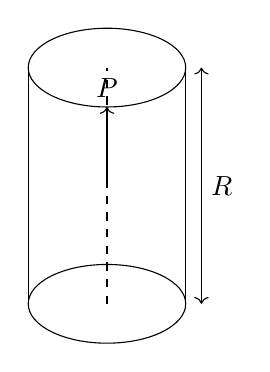
\begin{tikzpicture}
        \draw (0,0) ellipse (1 and 0.5);
        \draw (-1,0) -- (-1,3);
        \draw (1,0) -- (1,3);
        \draw (0,3) ellipse (1 and 0.5);
        \draw[->] (0,1.5) -- (0,2.5) node[above] {$\vv{P}$};
        \draw[dashed] (0,0) -- (0,3);
        \draw[<->] (1.2,0) -- (1.2,3) node[midway,right] {$R$};
    \end{tikzpicture}
    \item Thin ring:
    \begin{gather}
        J = \int_0^{2\pi} R^2 \lambda R \, d\theta = 2\pi R^3 \lambda = \boxed{m R^2}
    \end{gather}
    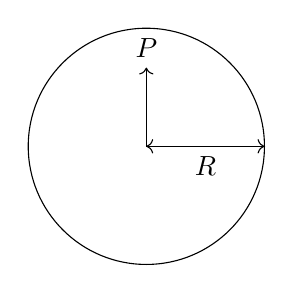
\begin{tikzpicture}
        \draw (0,0) circle (1.5);
        \draw[->] (0,0) -- (0,1) node[above] {$\vv{P}$};
        \draw[dashed] (0,0) -- (1.5,0);
        \draw[<->] (0,0) -- (1.5,0) node[midway,below] {$R$};
    \end{tikzpicture}
    \item Solid sphere:
    \begin{gather}
        J = \int_0^R r^2 \rho 4\pi r^2 \, dr = 4\pi\rho \left[ \frac{r^5}{5} \right]_0^R = \frac{4\pi\rho R^5}{5} = \boxed{\frac{2 m R^2}{5}}
    \end{gather}
    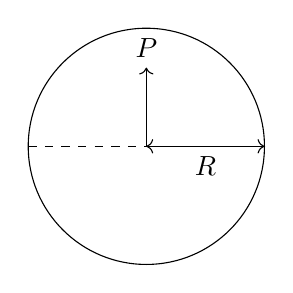
\begin{tikzpicture}
        \draw (0,0) circle (1.5);
        \draw[->] (0,0) -- (0,1) node[above] {$\vv{P}$};
        \draw[dashed] (-1.5,0) -- (1.5,0);
        \draw[<->] (0,0) -- (1.5,0) node[midway,below] {$R$};
    \end{tikzpicture}
    \item Cylindrical shell:
    \begin{gather}
        J = \int_{R_1}^{R_2} r^2 \sigma 2\pi r \, dr = 2\pi\sigma \left( \frac{R_2^4}{4} - \frac{R_1^4}{4} \right) = \boxed{\frac{m}{2} (R_1^2 + R_2^2)}
    \end{gather}
    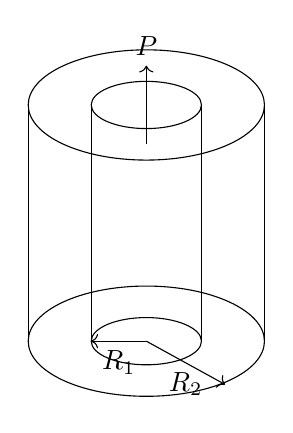
\begin{tikzpicture}
        \draw (0,0) ellipse (1.5 and 0.7);
        \draw (0,3) ellipse (1.5 and 0.7);
        \draw (-1.5,0) -- (-1.5,3);
        \draw (1.5,0) -- (1.5,3);
        \draw (0,0) ellipse (0.7 and 0.3);
        \draw (0,3) ellipse (0.7 and 0.3);
        \draw (-0.7,0) -- (-0.7,3);
        \draw (0.7,0) -- (0.7,3);
        \draw[->] (0,2.5) -- (0,3.5) node[above] {$\vv{P}$};
        \draw[<-] (-0.7,0) -- (0,0) node[midway,below] {$R_1$};
        \draw[->] (0,0) -- (1,-0.55) node[midway,below] {$R_2$};
    \end{tikzpicture}
    \item Thin rod (end axis):
    \begin{gather}
        J = \int_0^l r^2 \lambda \, dr = \lambda \left[ \frac{r^3}{3} \right]_0^l = \frac{\lambda l^3}{3} = \boxed{\frac{m l^2}{3}}
    \end{gather}
    \begin{tikzpicture}
        \draw[thick] (0,0) -- (4,0);
        \draw[->] (2,1) -- (2,2) node[above] {$\vv{P}$};
        \draw[dashed] (0,0) -- (0,1);
        \draw[<->] (0,-0.5) -- (4,-0.5) node[midway,below] {$l$};
        \draw[fill] (0,0) circle (0.05);
    \end{tikzpicture}
\end{enumerate}

\newpage

\section{Problem}
\noindent Prove that planetary orbits in the solar system are elliptical under Newtonian gravity.
\section*{Solution}
\setcounter{equation}{0}
\noindent We begin with Newton's law of gravitation and his second law of motion:
\begin{gather}
    \vv{F} = -\frac{GMm}{r^2}\vv{e_r} \quad \text{(Gravitational force)} \\
    \vv{F} = m\vv{a} \quad \text{(Newton's second law)}
\end{gather}
\noindent In polar coordinates $(r,\theta)$, the acceleration has two components:
\begin{gather}
    \vv{a} = (\ddot{r} - r\dot{\theta}^2)\vv{e_r} + (r\ddot{\theta} + 2\dot{r}\dot{\theta})\vv{e_\theta}
\end{gather}
\noindent Equating the components gives two equations of motion:
\begin{gather}
    \ddot{r} - r\dot{\theta}^2 = -\frac{GM}{r^2} \quad \text{(Radial equation)} \\
    r\ddot{\theta} + 2\dot{r}\dot{\theta} = 0 \quad \text{(Angular equation)}
\end{gather}
\noindent The angular equation can be rewritten as:
\begin{gather}
    \frac{1}{r}\frac{d}{dt}(r^2\dot{\theta}) = 0
\end{gather}
\noindent This implies conservation of angular momentum:
\begin{gather}
    L = r^2\dot{\theta} = \text{constant}
\end{gather}
\noindent To solve the radial equation, we make a substitution $u = 1/r$ and change variables using the chain rule:
\begin{gather}
    \dot{r} = \frac{dr}{dt} = \frac{dr}{d\theta}\dot{\theta} = -\frac{1}{u^2}\frac{du}{d\theta}\frac{L}{r^2} = -L\frac{du}{d\theta} \\
    \ddot{r} = -L\frac{d^2u}{d\theta^2}\dot{\theta} = -L^2u^2\frac{d^2u}{d\theta^2}
\end{gather}
\noindent Substituting into the radial equation:
\begin{gather}
    -L^2u^2\frac{d^2u}{d\theta^2} - \frac{L^2u^3}{u^2} = -GMu^2 \\
    \frac{d^2u}{d\theta^2} + u = \frac{GM}{L^2}
\end{gather}
\noindent This is an inhomogeneous second-order differential equation. The general solution is:
\begin{gather}
    u(\theta) = \frac{GM}{L^2} + A\cos(\theta - \theta_0)
\end{gather}
\noindent Converting back to $r$ and defining $e = AL^2/GM$:
\begin{gather}
    \boxed{r(\theta) = \frac{L^2/GM}{1 + e\cos(\theta - \theta_0)}}
\end{gather}
\noindent This is exactly the polar equation of a conic section with eccentricity $e$. \\
\noindent For planets, $0 \leq e < 1$, which corresponds to elliptical orbits.

\newpage

\section{Problem}
\setcounter{equation}{0}
Maxwell's Equations in Integral Form:
\begin{gather}
    \oint_S \vv{E} \cdot d\vv{S} = \frac{Q_{\text{enc}}}{\epsilon_0} \\
    \oint_S \vv{B} \cdot d\vv{S} = 0 \\
    \oint_L \vv{E} \cdot d\vv{l} = -\frac{d}{dt}\int_S \vv{B} \cdot d\vv{S} \\
    \oint_L \vv{B} \cdot d\vv{l} = \mu_0 I_{\text{enc}} + \mu_0\epsilon_0\frac{d}{dt}\int_S \vv{E} \cdot d\vv{S}
\end{gather}

\section{Problem}
\setcounter{equation}{0}
\begin{center}
\renewcommand{\arraystretch}{1.5} 
\setlength{\tabcolsep}{12pt}
\begin{tabular}{|l|l|l|l|}
\hline
Physical Quantity & Formula & Unit Symbol & SI Base Units \\ 
\hline
Current & $I = \frac{dQ}{dt}$ & A & A \\ 
\hline
Voltage & $V = IR$ & V & kg$\cdot$m$^2\cdot$s$^{-3}\cdot$A$^{-1}$ \\ 
\hline
Electric Charge & $Q = CV$ & C & A$\cdot$s \\ 
\hline
Capacitance & $C = \frac{Q}{V}$ & F & kg$^{-1}\cdot$m$^{-2}\cdot$s$^4\cdot$A$^2$ \\ 
\hline
Resistance & $R = \frac{V}{I}$ & $\Omega$ & kg$\cdot$m$^2\cdot$s$^{-3}\cdot$A$^{-2}$ \\ 
\hline
Conductance & $G = \frac{1}{R}$ & S & kg$^{-1}\cdot$m$^{-2}\cdot$s$^3\cdot$A$^2$ \\ 
\hline
Inductance & $V = L\frac{dI}{dt}$ & H & kg$\cdot$m$^2\cdot$s$^{-2}\cdot$A$^{-2}$ \\ 
\hline
Electric Field Strength & $\vv{E} = \frac{\vv{F}}{q}$ & V/m & kg$\cdot$m$\cdot$s$^{-3}\cdot$A$^{-1}$ \\ 
\hline
Magnetic Flux & $\Phi_B = \int \vv{B} \cdot d\vv{A}$ & Wb & kg$\cdot$m$^2\cdot$s$^{-2}\cdot$A$^{-1}$ \\ 
\hline
Magnetic Flux Density & $\vv{B} = \mu_0\vv{H} + \vv{M}$ & T & kg$\cdot$s$^{-2}\cdot$A$^{-1}$ \\ 
\hline
Electric Displacement Field & $\vv{D} = \epsilon_0\vv{E} + \vv{P}$ & C/m$^2$ & A$\cdot$s$\cdot$m$^{-2}$ \\ 
\hline
Magnetic Field Strength & $\vv{H} = \frac{\vv{B}}{\mu_0} - \vv{M}$ & A/m & A$\cdot$m$^{-1}$ \\ 
\hline
Permittivity & $\epsilon = \epsilon_0\epsilon_r$ & F/m & kg$^{-1}\cdot$m$^{-3}\cdot$s$^4\cdot$A$^2$ \\ 
\hline
Permeability & $\mu = \mu_0\mu_r$ & H/m & kg$\cdot$m$\cdot$s$^{-2}\cdot$A$^{-2}$ \\ 
\hline
Power & $P = VI$ & W & kg$\cdot$m$^2\cdot$s$^{-3}$ \\ 
\hline
Energy & $W = \int P\,dt$ & J & kg$\cdot$m$^2\cdot$s$^{-2}$ \\ 
\hline
Polarization Density & $\vv{P} = \epsilon_0\chi_e\vv{E}$ & C/m$^2$ & A$\cdot$s$\cdot$m$^{-2}$ \\ 
\hline
Magnetization & $\vv{M} = \chi_m\vv{H}$ & A/m & A$\cdot$m$^{-1}$ \\ 
\hline
\end{tabular}
\end{center}

\newpage

\section{Problem}
\setcounter{equation}{0}
\begin{table}[h]
\centering
\begin{tabular}{>{\raggedright\arraybackslash}p{5cm}p{7cm}}
\toprule
\textbf{Charge Distribution} & \textbf{Electric Field} \\
\midrule
Point charge with charge $q$ & 
\[ E = \frac{q}{4 \pi \epsilon_0 r^2} \] \\
\addlinespace
Uniformly charged spherical shell with radius $R$ and charge $q$ & 
\[ E = 
\begin{cases} 
0, & \text{inside the sphere} \\ 
\frac{q}{4 \pi \epsilon_0 r^2}, & \text{outside the sphere} 
\end{cases} \] \\
\addlinespace
Uniformly charged solid sphere with radius $R$ and charge $q$ & 
\[ E = 
\begin{cases} 
\frac{qr}{4 \pi \epsilon_0 R^3}, & \text{inside the sphere} \\ 
\frac{q}{4 \pi \epsilon_0 r^2}, & \text{outside the sphere} 
\end{cases} \] \\
\addlinespace
Infinitely long uniformly charged line with linear charge density $\lambda$ & 
\[ E = \frac{\lambda}{2 \pi \epsilon_0 r} \] \\
\addlinespace
Infinitely large uniformly charged plane with surface charge density $\sigma$ & 
\[ E = \frac{\sigma}{2 \epsilon_0} \] \\
\bottomrule
\end{tabular}
\end{table}

\newpage

\section{Problem}
The air resistance is given by $\vv{F}_r = -k\vv{v}$. \\
Find the trajectory equation for a projectile with mass $m$, initial velocity $\vv{v}_0$, and projection angle $\alpha$.
\section*{Solution}
\begin{center}
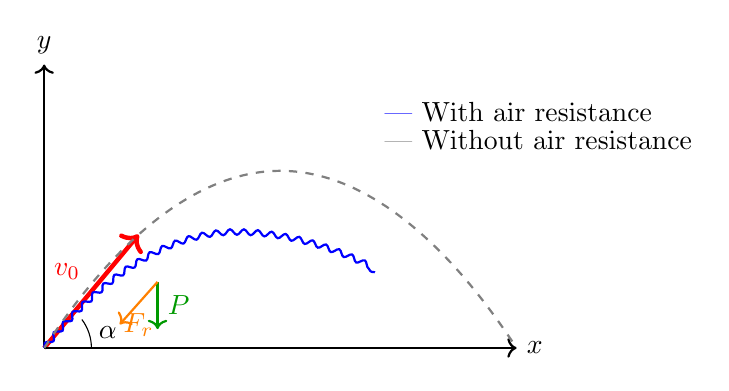
\begin{tikzpicture}[scale=1.2]
    \draw[->, thick] (0,0) -- (5,0) node[right]{$x$};
    \draw[->, thick] (0,0) -- (0,3) node[above]{$y$}; 
    \draw[->, ultra thick, red] (0,0) -- (1,1.2) node[midway, above left]{$\vv{v}_0$};
    \draw[dashed] (0,0) -- (2,0);
    \draw (0.5,0) arc (0:37:0.5) node[midway, right]{$\alpha$};   
    \draw[blue, thick, decorate, decoration={snake, amplitude=1pt, segment length=5pt}] 
        (0,0) parabola bend (2,1.2) (3.5,0.8); 
    \draw[gray, dashed, thick] (0,0) parabola bend (2.5,1.875) (5,0); 
    \draw[->, thick, green!60!black] (1.2,0.7) -- (1.2,0.2) node[midway, right]{$\vv{P}$};
    \draw[->, thick, orange] (1.2,0.7) -- (0.8,0.25) node[midway, below]{$\vv{F}_r$};   
    \draw (3.5,2.5) node[right]{\textcolor{blue}{---} With air resistance};
    \draw (3.5,2.2) node[right]{\textcolor{gray}{---} Without air resistance};
\end{tikzpicture}
\end{center}
\subsection*{Horizontal Motion}
\setcounter{equation}{0}
\begin{gather}
    m\frac{\mathrm{d}v_x}{\mathrm{d}t} = -kv_x \\ 
    \frac{\mathrm{d}v_x}{v_x} = -\frac{k}{m}\mathrm{d}t \\ 
    \ln v_x = -\frac{k}{m}t + C \\
    v_x = v_{0x}e^{-kt/m} = v_0\cos\alpha\cdot e^{-kt/m} \\
    x = \int_0^t v_x \mathrm{d}t = \frac{mv_0\cos\alpha}{k}\left(1 - e^{-kt/m}\right)
\end{gather}
\subsection*{Vertical Motion}
\begin{gather}
    m\frac{\mathrm{d}v_y}{\mathrm{d}t} = -mg - kv_y \\
    \frac{\mathrm{d}v_y}{v_y + mg/k} = -\frac{k}{m}\mathrm{d}t \\
    \ln\left(v_y + \frac{mg}{k}\right) = -\frac{k}{m}t + C \\
    v_y = \left(v_0\sin\alpha + \frac{mg}{k}\right)e^{-kt/m} - \frac{mg}{k} \\
    y = \int_0^t v_y \mathrm{d}t = \frac{m}{k}\left(v_0\sin\alpha + \frac{mg}{k}\right)\left(1 - e^{-kt/m}\right) - \frac{mg}{k}t
\end{gather}
\subsection*{Eliminating Time Parameter}
\begin{gather}
    e^{-kt/m} = 1 - \frac{kx}{mv_0\cos\alpha} \\
    t = -\frac{m}{k}\ln\left(1 - \frac{kx}{mv_0\cos\alpha}\right)
\end{gather}
\subsection*{Final Result}
\begin{gather}
    \boxed{y = \left(\tan\alpha + \frac{mg}{kv_0\cos\alpha}\right)x + 
    \frac{m^2g}{k^2}\ln\left(1 - \frac{kx}{mv_0\cos\alpha}\right)}
\end{gather}

\newpage

\section{Problem}
Given: Light rope of length $l$, mass $m$ at one end, fixed at point $O$. \\
Initial position: lowest point with initial horizontal velocity $\vv{v_0}$. \\
Calculate both the instantaneous speed of the pendulum bob and the corresponding cord tension 
at any point during its circular motion.
\section*{Solution}
\begin{center}
\begin{tikzpicture}[scale=1.5,>=Stealth]
    \coordinate (O) at (0,0);
    \fill (O) circle (1.5pt) node[above] {$O$};
    \draw[dashed] (O) circle (2cm);
    \coordinate (initial) at (0,-2);
    \filldraw (initial) circle (1.5pt) node[below=3pt] {Initial position};
    \draw[->,thick,green!70!black] (initial) -- +(1,0) node[midway,above] {$\vv{v_0}$};
    \def\theta{60} 
    \coordinate (mass) at ($(O)+(270+\theta:2)$);
    \filldraw (mass) circle (1.5pt) node[above right] {$m$};
    \draw (O) -- (mass) node[midway,above right] {$l$};
    \draw[->,red,thick] (mass) -- ($(mass)!0.7!(O)$) node[above left] {$\vv{F_T}$};
    \draw[->,blue,thick] (mass) -- +(0,-1) node[right] {$\vv{P}$};
    \draw[->,thick] (mass) -- +(\theta:1) node[above right] {$\vv{v}$};
\end{tikzpicture}
\end{center}
\setcounter{equation}{0}
Using differential work-energy principle:
\begin{gather}
    \dd{W} = \dd{T} + \dd{U} \\
    \vv{P}\cdot\dd{\vv{r}} = \dd\left(\frac{1}{2}m\vv{v}\cdot\vv{v}\right) + \dd(mgy) \\
    -mg\dd{y} = m\vv{v}\cdot\dd{\vv{v}} + mg\dd{y} \\
    \int_{v_0}^v v\dd{v} = -g\int_{0}^{l(1-\cos\theta)} \dd{y} \\
    \frac{1}{2}(v^2 - v_0^2) = -gl(1-\cos\theta) \\
    v^2 = v_0^2 - 2gl(1-\cos\theta)
\end{gather}
Radial dynamics using polar coordinates:
\begin{gather}
    \sum F_r = -F_T + P_r = m\ddot{r} - mr\dot{\theta}^2 \\
    -F_T + mg\cos\theta = -ml\dot{\theta}^2 \quad (\text{since } r = l \text{ constant}) \\
    F_T = m\left(g\cos\theta + l\dot{\theta}^2\right) \\
    \text{Using } v = l\dot{\theta} \text{ and energy result:} \\
    F_T = m\left(g\cos\theta + \frac{v_0^2}{l} - 2g(1-\cos\theta)\right)
\end{gather}
\begin{gather}
    \boxed{v = \sqrt{v_0^2 + 2gl(\cos\theta - 1)}} \\
    \boxed{F_T= m\left(\frac{v_0^2}{l} - 2g + 3g\cos\theta\right)}
\end{gather}

\newpage

\section{Problem}
A flexible chain of length $l$ and linear mass density $\lambda$ lies on a table with a small hole. \\
One end of the chain hangs slightly down through the hole, while the rest is piled around it. \\
Due to a disturbance, the chain starts to fall under its own weight. \\
Neglecting friction, find the relationship between the velocity $v$ and the falling distance $y$.
\section*{Solution}
\setcounter{equation}{0}
\begin{figure}[h]
\centering
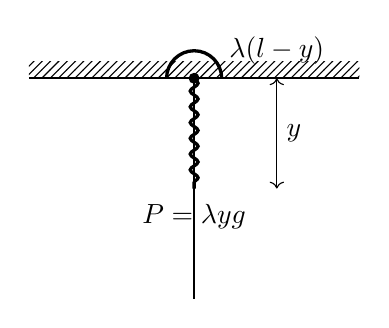
\begin{tikzpicture}[scale=0.7]
\draw[thick] (-3,0) -- (3,0);
\fill[pattern=north east lines] (-3,0) rectangle (3,0.3);
\draw[thick] (0,0) -- (0,-4);
\fill (0,0) circle (0.1);
\draw[very thick,decorate,decoration={snake,amplitude=0.5mm,segment length=2mm}] (0,0) -- (0,-2);
\draw[very thick] (0.5,0) arc (0:180:0.5);
\draw[<->] (1.5,0) -- (1.5,-2) node[midway,right]{$y$};
\node at (0,-2.5) {$\vv{P} = \lambda y \vv{g}$};
\node at (1.5,0.5) {$\lambda(l-y)$};
\end{tikzpicture}
\end{figure}
\begin{gather}
\frac{d}{dt}(\lambda y v) = \lambda y g \implies \lambda v \frac{dy}{dt} + \lambda y \frac{dv}{dt} = \lambda y g \\
v^2 + y v \frac{dv}{dy} = y g \\
\text{Let } v^2 = u \Rightarrow u + \frac{y}{2} \frac{du}{dy} = y g \\
\frac{d}{dy}(u y^2) = 2g y^3 \implies u y^2 = \frac{g y^4}{2} \\
\boxed{v = \left(\frac{2gy}{3}\right)^{1/2}}
\end{gather}
\subsection*{Method 1: Direct Integration}
\begin{gather}
\int_0^t \lambda y g dt = \lambda y v \nonumber \\
g\int_0^y y dy = \int_0^v y v dy \nonumber \\
\frac{1}{2}gy^2 = \frac{1}{3}y v^2 \nonumber \\
\boxed{v = \left(\frac{2gy}{3}\right)^{1/2}}
\end{gather}
\subsection*{Method 2: Energy Conservation}
\begin{gather}
\lambda y g dy = \frac{1}{2}\lambda d(y v^2) \nonumber \\
g y dy = \frac{1}{2}d(y v^2) \nonumber \\
\frac{1}{2}gy^2 = \frac{1}{2}y v^2 \nonumber \\
\boxed{v = \left(\frac{2gy}{3}\right)^{1/2}}
\end{gather}

\newpage

\section{Problem}
A smooth ring with radius $R$ is placed in a vertical plane.\\
A small ball with mass $m$ slides on the ring and can move freely without friction.\\
The ball starts from rest at point $A$.\\
Find the angular velocity $\omega$ of the ball about $O$ when it reaches point $B$.
\section*{Solution}
\setcounter{equation}{0}
\begin{center}
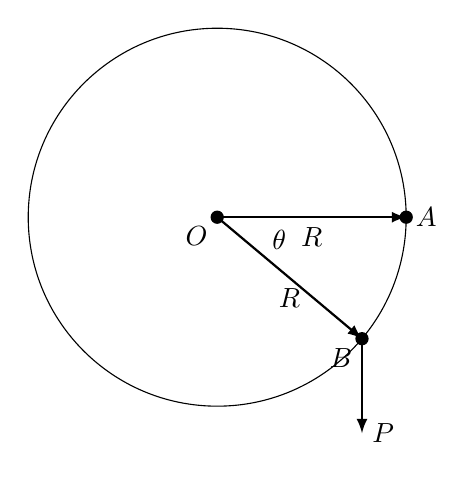
\begin{tikzpicture}[scale=1.2]
    \draw (0,0) circle (2cm);
    \coordinate (O) at (0,0);
    \coordinate (A) at (2,0);
    \coordinate (B) at (320:2cm); 
    \fill (O) circle (2pt) node[below left] {$O$};
    \fill (A) circle (2pt) node[right] {$A$};
    \fill (B) circle (2pt) node[below left] {$B$};  
    \draw[-latex,thick] (O) -- (A) node[midway,below] {$R$};
    \draw[-latex,thick] (O) -- (B) node[midway,below] {$R$};
    \node at (340:0.7) {$\theta$};
    \draw[-latex,thick] (B) -- ++(0,-1) node[right] {$\vv{P}$};
\end{tikzpicture}
\end{center}
\subsection*{Method 1: Energy Conservation}
\begin{gather}
\Delta h = R\sin\theta \\
\frac{1}{2}mv^2 = mg\Delta h \\
v^2 = 2gR\sin\theta \\
v = R\omega \\
\boxed{\omega = \sqrt{\frac{2g\sin\theta}{R}}}
\end{gather}
\subsection*{Method 2: Calculus Approach}
\begin{gather}
\vv{P} = m\vv{g} \\
\text{Tangential component: } P_\tau = -mg\sin\phi \quad \text{(angle $\phi$ measured from horizontal axis)} \\
\tau = P_\tau R = -mgR\sin\phi \\
I\alpha = \tau \Rightarrow mR^2\frac{d\omega}{dt} = -mgR\sin\phi \\
\frac{d\omega}{dt} = -\frac{g}{R}\sin\phi \\
\omega\frac{d\omega}{d\phi} = -\frac{g}{R}\sin\phi \quad \text{(chain rule)} \\
\int_0^\omega \omega\,d\omega = -\frac{g}{R}\int_0^\theta \sin\phi\,d\phi  \\
\frac{\omega^2}{2} = \frac{g}{R}(\cos\theta - 1) \\
\text{From geometry: } \cos\theta = 1 - \sin\theta \\
\boxed{\omega = \sqrt{\frac{2g\sin\theta}{R}}}
\end{gather}

\newpage

\section{Problem}
A uniform rod of length $l$ and mass $m'$ can rotate freely about pivot O.\\
 A bullet of mass $m$ with initial velocity $\vv{v}$ hits the rod at distance $a$ from O, \\
 causing the rod to swing to a maximum angle of 30$^\circ$. \\
Find the initial speed $v$ of the bullet.
\section*{Solution}
\setcounter{equation}{0}
\begin{figure}[h]
\centering
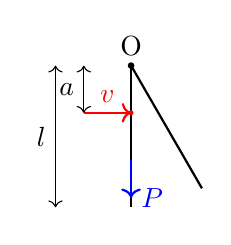
\begin{tikzpicture}[scale=0.6]
    \fill (0,3) circle (2pt) node[above] {O};
    \draw[thick] (0,3) -- (0,0);
    \draw[thick,rotate around={30:(0,3)}] (0,3) -- (0,0);
    \fill[red] (0,2) circle (1.5pt);
    \draw[red,->,thick] (-1,2) -- (0,2) node[midway,above] {$\vv{v}$};
    \draw[<->] (-1,3) -- (-1,2) node[midway,left] {$a$};
    \draw[<->] (-1.6,3) -- (-1.6,0) node[midway,left] {$l$};
    \draw[->,thick,blue] (0,1) -- (0,0.2) node[right] {$\vv{P}$};
\end{tikzpicture}
\end{figure}
\begin{gather}
mva = \left(\frac{1}{3}m'l^2 + ma^2\right)\omega \\
\frac{1}{2}\left(\frac{1}{3}m'l^2 + ma^2\right)\omega^2 = \left(\frac{m'l}{2} + ma\right)g(1 - \cos30^\circ) 
\end{gather}
\begin{gather}
\boxed{v = \sqrt{(2-\sqrt{3})(m'l+2ma)(m'l^2+3ma^2)g/6} \big/ ma}
\end{gather}

\section{Problem}
Two long parallel straight wires with radius \( R \), the distance between their centers is \( d \) (\( d \gg R \)).\\
Find the capacitance per unit length of the wires.
\section*{Solution}
\setcounter{equation}{0}
\begin{figure}[h]
\centering
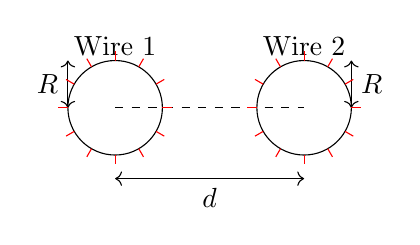
\begin{tikzpicture}[scale=0.6]
    \draw (0,0) circle (1cm);
    \draw (4,0) circle (1cm);
    \draw[dashed] (0,0) -- (4,0);
    \node at (0,1.3) {Wire 1};
    \node at (4,1.3) {Wire 2};
    \draw[<->] (0,-1.5) -- node[below] {\( d \)} (4,-1.5);
    \draw[<->] (-1,0) -- node[left] {\( R \)} (-1,1);
    \draw[<->] (5,0) -- node[right] {\( R \)} (5,1);
    \foreach \x in {0,30,...,330} {
        \draw[red] (0,0) ++(\x:1cm) -- ++(\x:0.2cm);
        \draw[red] (4,0) ++(\x+180:1cm) -- ++(\x+180:0.2cm);
    }
\end{tikzpicture}
\caption{Cross-section of two parallel wires with charge distributions}
\end{figure}
For a single wire with charge \( \lambda \) per unit length, the potential at distance \( r \) is:
\begin{gather}
    V = \frac{\lambda}{2\pi\epsilon_0} \ln\left(\frac{r_0}{r}\right)
\end{gather}
For two wires with opposite charges \( \pm\lambda \), the potential difference is:
\begin{gather}
    U = V_+ - V_- = \frac{\lambda}{2\pi\epsilon_0} \left[\ln\left(\frac{r_0}{R}\right) - \ln\left(\frac{r_0}{d-R}\right)\right] \\
    U = \frac{\lambda}{2\pi\epsilon_0} \ln\left(\frac{d-R}{R}\right) \approx \frac{\lambda}{2\pi\epsilon_0} \ln\left(\frac{d}{R}\right) \quad (\text{since } d \gg R)
\end{gather}
\begin{gather}
    \boxed{C_l = \frac{\lambda}{U} \approx \frac{\pi\epsilon_0}{\ln(d/R)}}
\end{gather}

\newpage

\section{Problem}
A long straight cylindrical conductor with radius $R_1$ and a coaxial thin cylindrical conductor shell with radius $R_2$ are separated by air.\\
The line charge densities are $+\lambda$ and $-\lambda$ respectively. Given the breakdown field strength of air $E_b$,\\ 
find the maximum $R_1$ that maximizes the stored energy without causing air breakdown.
\section*{Solution}
\setcounter{equation}{0}
\begin{center}
\tdplotsetmaincoords{85}{110}
\begin{tikzpicture}[scale=1.4, tdplot_main_coords]
    \draw[thick,->] (0,0,0) -- (6,0,0) node[anchor=north east]{$x$};
    \draw[thick,->] (0,0,0) -- (0,3,0) node[anchor=north west]{$y$};
    \draw[thick,->] (0,0,0) -- (0,0,3) node[anchor=south]{$z$};
    \begin{scope}[canvas is xy plane at z=-2]
        \filldraw[gray!30, opacity=0.7] (0,0) circle (1cm);
        \draw[thick] (0,0) circle (1cm);
    \end{scope}
    \begin{scope}[canvas is xy plane at z=2]
        \filldraw[gray!30, opacity=0.7] (0,0) circle (1cm);
        \draw[thick] (0,0) circle (1cm);
    \end{scope}
    \draw[thick] (1,0,-2) -- (1,0,2);
    \draw[thick] (-1,0,-2) -- (-1,0,2);
    \node at (0,0.2,0.2) {\scriptsize $+\lambda$};
    \begin{scope}[canvas is xy plane at z=-2]
        \draw[thick] (0,0) circle (2cm);
    \end{scope}
    \begin{scope}[canvas is xy plane at z=2]
        \draw[thick] (0,0) circle (2cm);
    \end{scope}
    \draw[thick] (2,0,-2) -- (2,0,2);
    \draw[thick] (-2,0,-2) -- (-2,0,2);
    \node at (1.5,0,-0.2) {\scriptsize $-\lambda$};
    \foreach \z in {-1.8,-1.2,...,1.8} {
        \foreach \angle in {0,45,...,315} {
            \draw[blue,->] (\angle:1.1) -- (\angle:1.9);
            \begin{scope}[shift={(0,0,\z)}]
                \draw[blue,->] (\angle:1.1) -- (\angle:1.9);
            \end{scope}
        }
    }
    \draw[thick, dashed] (0,0,-2.5) -- (0,0,2.5) node[right]{Axis};
    \draw[thick,->] (0,0,0) -- (1,0,0) node[midway,below]{\scriptsize $R_1$};
    \draw[thick,->] (0,0,1.5) -- (2,0,1.5) node[midway,above]{\scriptsize $R_2$};
\end{tikzpicture}
\end{center}
\begin{gather}
    \vv{E}(r) = \frac{\lambda}{2\pi\epsilon_0 r} \hat{r} \quad (R_1 < r < R_2) \\
    \text{At } r = R_1: \quad E_{\text{max}} = \frac{\lambda}{2\pi\epsilon_0 R_1} \leq E_b \\
    \lambda_{\text{max}} = 2\pi\epsilon_0 R_1 E_b \\
    V = \int_{R_1}^{R_2} \vv{E} \cdot d\vv{r} = \frac{\lambda}{2\pi\epsilon_0} \ln\left(\frac{R_2}{R_1}\right) \\
    C = \frac{\lambda}{V} = \frac{2\pi\epsilon_0}{\ln(R_2/R_1)} \\
    U = \frac{1}{2}CV^2 = \frac{\lambda^2}{4\pi\epsilon_0}\ln\left(\frac{R_2}{R_1}\right) \\
    \text{Substitute } \lambda_{\text{max}}: \quad U(R_1) = \pi\epsilon_0 E_b^2 R_1^2 \ln\left(\frac{R_2}{R_1}\right) \\
    \frac{dU}{dR_1} = 2\pi\epsilon_0 E_b^2 R_1 \ln\left(\frac{R_2}{R_1}\right) - \pi\epsilon_0 E_b^2 R_1 = 0 \\
    \ln\left(\frac{R_2}{R_1}\right) = \frac{1}{2} \Rightarrow R_1 = \frac{R_2}{\sqrt{e}} \\
    \text{With breakdown condition:} \quad R_1^{\text{max}} = \boxed{\frac{E_b R_2}{2\sqrt{e}}}
\end{gather}

\newpage

\section{Problem}
A metal cylindrical shell with inner radius $R_1$, outer radius $R_2$, length $l$, \\
and resistivity $\rho$. If the inner edge has higher potential than the outer edge, \\
when the potential difference is $U$, what is the radial current in the cylinder?
\section*{Solution}
\setcounter{equation}{0}
\begin{figure}[h]
\centering
\tdplotsetmaincoords{75}{110}
\begin{tikzpicture}[scale=1.8,tdplot_main_coords]
    \draw[->] (0,0,0) -- (3,0,0) node[anchor=north east]{$x$};
    \draw[->] (0,0,0) -- (0,2,0) node[anchor=north west]{$y$};
    \draw[->] (0,0,0) -- (0,0,3) node[anchor=south]{$z$};
    \draw[thick] (0,0,0) circle (1);
    \draw[thick] (0,0,2) circle (1);
    \draw[thick] (1,0,0) -- (1,0,2);
    \draw[thick] (-1,0,0) -- (-1,0,2);
    \draw[thick] (0,1,0) -- (0,1,2);
    \draw[thick] (0,-1,0) -- (0,-1,2);
    \draw[thick,dashed] (0,0,0) circle (1.5);
    \draw[thick] (0,0,2) circle (1.5);
    \draw[thick] (1.5,0,0) -- (1.5,0,2);
    \draw[thick] (-1.5,0,0) -- (-1.5,0,2);
    \draw[thick] (0,1.5,0) -- (0,1.5,2);
    \draw[thick] (0,-1.5,0) -- (0,-1.5,2);
    \draw[->,>=stealth] (0,0,2.2) -- (0,0,0.2) node[midway,right]{$l$};
    \draw[->,>=stealth] (0,0,0) -- (0.707,-0.707,0) node[midway,above left]{$R_1$};
    \draw[->,>=stealth] (0,0,0) -- (0,1.5,0) node[midway,above left]{$R_2$};
    \foreach \z in {0,0.4,0.8,1.2,1.6,2.0}
    \draw[->,red,thick] (1.1,0,\z) -- (1.4,0,\z);
\end{tikzpicture}
\end{figure}
Consider a thin cylindrical shell at radius $r$ with thickness $dr$:
\begin{gather}
    dR = \rho \frac{dr}{A} = \rho \frac{dr}{2\pi r l} \\
    R = \int_{R_1}^{R_2} dR = \frac{\rho}{2\pi l} \int_{R_1}^{R_2} \frac{dr}{r} = \frac{\rho}{2\pi l} \ln\left(\frac{R_2}{R_1}\right) \\
    \boxed{I = \frac{U}{R} = \frac{U}{\frac{\rho}{2\pi l} \ln\left(\frac{R_2}{R_1}\right)} = \frac{2\pi l U}{\rho \ln(R_2/R_1)}}
\end{gather}

\newpage

\section{Problem}
The magnetic field of a current-carrying straight wire. \\
In vacuum, there is a long straight wire CD carrying current $I$. \\
Find the magnetic induction $\vv{B}$ at an arbitrary point P near the wire. \\
The perpendicular distance between point P and the wire is $r_0$.

\section*{Solution}
\setcounter{equation}{0}
\begin{center}
\begin{tikzpicture}[scale=1.5, >=Stealth]
    \tdplotsetmaincoords{75}{120}
    \begin{scope}[tdplot_main_coords]
        \draw[thick, ->] (0,0,-2) -- (0,0,2) node[below left]{$CD$};
        \draw[thick] (0,0,-2.5) -- (0,0,2.5);
        \foreach \z in {-1.5,0,1.5} {
            \draw[->, orange!80!black] (0.2,0,\z) -- (0.6,0,\z);}
        \node at (0.9,0,0) {$I$};
        \coordinate (P) at (2,0,0);
        \fill[red] (P) circle (1.5pt) node[above right]{$P$};
        \draw[dashed, green!50!black] (0,0,0) -- (P) node[midway, above]{$r_0$};
        \coordinate (dl) at (0,0,0.7);
        \draw[very thick, blue] (dl) -- ++(0,0,0.1) node[right]{$d\vv{l}$};
        \draw[->, thick, purple] (dl) -- (P) node[midway, below]{$\vv{r}$};
        \draw[->, cyan] (0,0,0) -- (3,0,0) node[below left]{$x$};
        \draw[->, cyan] (0,0,0) -- (0,2,0) node[below left]{$y$};
        \draw[->, cyan] (0,0,0) -- (0,0,3) node[below left]{$z$};
        \draw[orange, dashed] (0,0,0.7) -- (2,0,0.7);
        \draw[orange, dashed] (2,0,0.7) -- (P);
        \coordinate (origin) at (0,0,0.7);
        \pic[draw, <->, red, angle radius=0.8cm, angle eccentricity=1.3, 
             "$\theta$"] {angle = P--origin--dl};
        \draw[->, thick, magenta] (P) -- ++(0,0.8,0) node[above]{$\vv{B}$};
    \end{scope}
\end{tikzpicture}
\end{center}
\begin{gather}
d\vv{B} = \frac{\mu_0}{4\pi} \frac{I d\vv{l} \times \vv{r}}{r^3} \\
|\vv{dB}| = \frac{\mu_0}{4\pi} \frac{I dl \sin\theta}{r^2} \\
\text{From geometry: } r = \frac{r_0}{\sin\theta}, \quad l = -r_0 \cot\theta \\
dl = \frac{r_0}{\sin^2\theta} d\theta \\
\text{Substituting into the integral:} \\
B = \frac{\mu_0 I}{4\pi} \int_{-\infty}^{\infty} \frac{dl \sin\theta}{r^2} = 
    \frac{\mu_0 I}{4\pi} \int_{0}^{\pi} \frac{(r_0 d\theta / \sin^2\theta) \sin\theta}{(r_0^2 / \sin^2\theta)} \\
B = \frac{\mu_0 I}{4\pi r_0} \int_{0}^{\pi} \sin\theta d\theta \\
B = \frac{\mu_0 I}{4\pi r_0} [-\cos\theta]_{0}^{\pi} = \frac{\mu_0 I}{4\pi r_0} (1 - (-1)) \\
\boxed{B = \frac{\mu_0 I}{2\pi r_0}}
\end{gather}

\newpage

\section{Problem}
Electromagnetic catapult principle: Two parallel cylindrical conductor rails with length $L$, radius $R$, and separation $d$ ($L \gg d$). \\
A rod-shaped metal projectile of mass $m$ connects the rails, forming a circuit with external power supply carrying current $I$. \\
(1) Find the magnetic force on the projectile.\\
(2) If the projectile starts from the middle of the rails with acceleration distance $L/2$, find its exit velocity.
\section*{Solution}
\setcounter{equation}{0}
\begin{gather}
\begin{aligned}
&\text{(1) The magnetic field at distance } r \text{ from a single wire:} \\
&\boxed{B = \frac{\mu_0 I}{2\pi r}} \\
&\text{Force on the projectile:} \\
&\vv{F} = I \int_{R}^{R+d} \vv{dl} \times \vv{B} \\
&F = \frac{\mu_0 I^2}{2\pi} \ln\left(\frac{R+d}{R}\right) \\
&\text{(2) Using work-energy theorem:} \\
&\frac{1}{2}mv^2 = F \cdot \frac{L}{2} \\
&\boxed{v = \sqrt{\frac{\mu_0 I^2 L}{2\pi m} \ln\left(\frac{R+d}{R}\right)}}
\end{aligned}
\end{gather}
\begin{figure}[h]
\centering
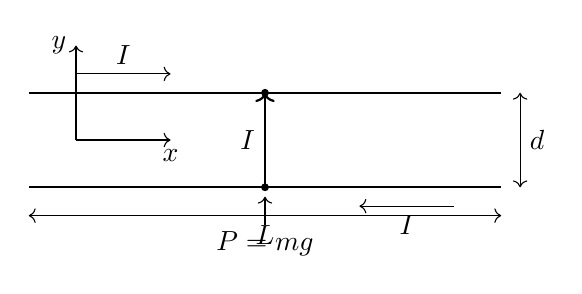
\begin{tikzpicture}[scale=1.2]
    \draw[thick] (0,0) -- (5,0);
    \draw[thick] (0,1) -- (5,1);
    \draw[thick,->] (2.5,0) -- (2.5,1) node[midway,left] {$I$};
    \filldraw (2.5,0) circle (1pt);
    \filldraw (2.5,1) circle (1pt);
    \draw[<->] (5.2,0) -- (5.2,1) node[midway,right] {$d$};
    \draw[<->] (0,-0.3) -- (5,-0.3) node[midway,below] {$L$};
    \node at (2.5,-0.6) {$\vv{P} = m\vv{g}$};
    \draw[->] (2.5,-0.4) -- (2.5,-0.1);
    \draw[->] (0.5,1.2) -- (1.5,1.2) node[midway,above] {$I$};
    \draw[->] (4.5,-0.2) -- (3.5,-0.2) node[midway,below] {$I$}; 
    \draw[->] (0.5,0.5) -- (1.5,0.5) node[below] {$x$};
    \draw[->] (0.5,0.5) -- (0.5,1.5) node[left] {$y$};
\end{tikzpicture}
\end{figure}

\newpage

\end{document}